\subsection{Traffic Filtering}

\begin{frame}{current solutions}
	\begin{itemize}
		\item The Networking stack can filter \textbf{egress} and \textbf{ingress} traffic
			\begin{itemize}
				\item Necessary for \textbf{firewalling}
			\end{itemize}
		\item Filters can also identify \textbf{packets of interest} for on-the-fly modification
			\begin{itemize}
				\item e.g. NAT : The destination \textbf{IPv4} address is re-written
			\end{itemize}
		\item Historically, multiple solutions have been implemented in the Linux Kernel :
			\begin{itemize}
				\item \code{iptables} and \code{ip6tables} for Layer 3
				\item \code{arptables} and \code{ebtables} for Layers 2 and 3
				\item These solutions have been replaced by \textbf{netfilter} and its \textbf{nftables}
			\end{itemize}
		\item Alternative solutions exist :\textbf{eBPF}, \textbf{P4} and \textbf{TC}
	\end{itemize}
\end{frame}

\begin{frame}{Legacy filtering solutions}
	\begin{itemize}
		\item There used to be multiple traffic filtering, each for a different layer
		\item \code{iptables} and \code{ip6tables} : IP-level filtering and mangling
			\begin{itemize}
				\item \kfile{net/ipv4/netfilter/ip_tables.c} and \kfile{net/ipv6/netfilter/ip6_tables.c}
			\end{itemize}
		\item \code{ebtables} : Filtering based on Layer 2 information
			\begin{itemize}
				\item Filter and forward VLANs and bridging operations
				\item ARP filtering
			\end{itemize}
	\end{itemize}
\end{frame}

\begin{frame}{nftables}
	\begin{itemize}
		\item Originates from the \href{https://www.netfilter.org/}{Netfilter project}
		\item More modern approach, with a centralized filtering table and multiple \textbf{hooks}
		\item Rules expressed in a low-level language
		\item Users attach \textbf{chains} to \textbf{hooks} to express rules
		\item Chains are stored within \textbf{tables} created by users
		\item See the \href{https://wiki.nftables.org/wiki-nftables/index.php/Simple_ruleset_for_a_server}{project provided examples}
	\end{itemize}
\end{frame}

\begin{frame}{Netfilter hooks}
	\begin{columns}
		\column{0.4\textwidth}
		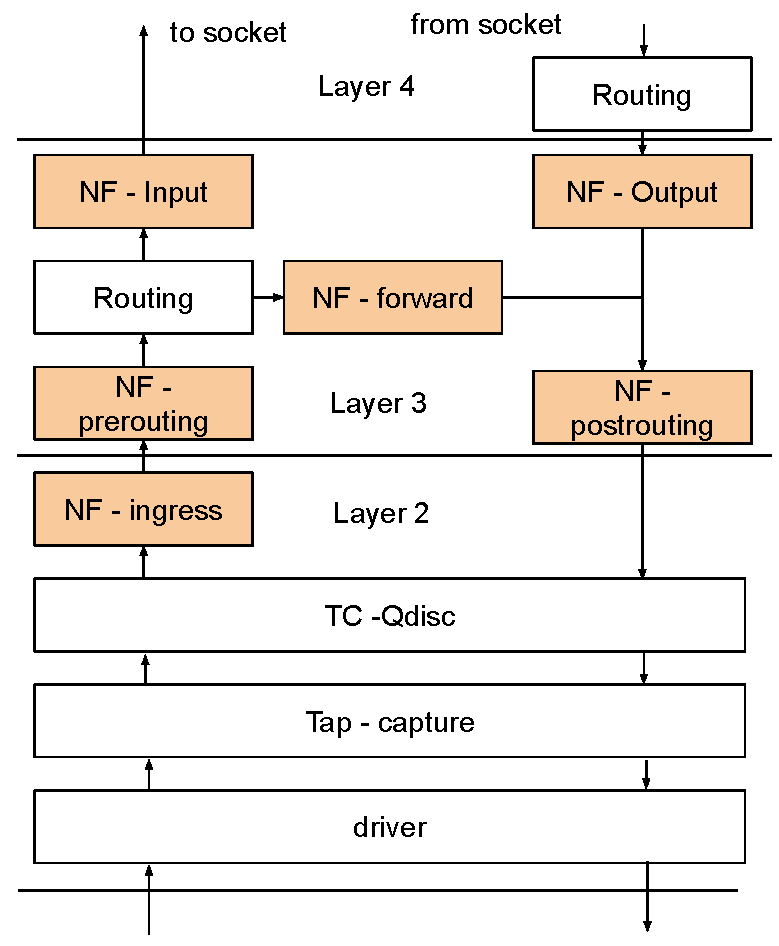
\includegraphics[width=1\textwidth]{slides/networking-filtering/routing_nf.pdf}
		\column{0.6\textwidth}
		\begin{itemize}
			\item \textbf{ingress} : Filter as soon as the packet is received
			\item \textbf{pre-routing} : Filter before taking a routing decision
			\item \textbf{input} : Filter packets going to sockets
			\item \textbf{forward} : Filter packets forwarded to the outside
			\item \textbf{output} : Filter local outgoing packets
			\item \textbf{post-routing} : Filter all outgoing packets
		\end{itemize}
	\end{columns}
\end{frame}

\begin{frame}{netfilter in userspace}
	\begin{itemize}
		\item Netfilter was integrated as another backed for existing tools like \textbf{iptables}
		\item Dedicated tool is called \textbf{nft}, see \manpage{nft}{8}
	\end{itemize}
\end{frame}


